\documentclass[11pt]{article}
\usepackage[margin=1in]{geometry}
\usepackage{mathpazo}
\usepackage{amsmath,amssymb}
\usepackage{microtype}
\usepackage{booktabs}
\usepackage{graphicx}
\usepackage[dvipsnames]{xcolor}
\usepackage{tikz}
\usetikzlibrary{positioning,arrows.meta,calc,fit,backgrounds,decorations.pathreplacing}
\usepackage[most]{tcolorbox}
\usepackage{enumitem}
\usepackage{listings}
\usepackage[font=small,labelfont=bf]{caption}
\usepackage{hyperref}
\hypersetup{colorlinks=true,linkcolor=MidnightBlue,citecolor=MidnightBlue,urlcolor=MidnightBlue}
\usepackage{cleveref}
\urlstyle{tt}
\def\UrlBreaks{\do\_\do/\do.}
\newcommand{\file}[1]{\nolinkurl{#1}}
\newcommand{\code}[1]{\texttt{#1}}
\newcommand{\mhh}{m_{hh}}
\newcommand{\bC}{\boldsymbol{C}}

\definecolor{trainable}{HTML}{1B6CA8}
\definecolor{physics}{HTML}{2E933C}
\definecolor{datac}{HTML}{7B4EA3}
\definecolor{warn}{HTML}{C0392B}

\newtcolorbox{keyidea}[1][]{enhanced,breakable,colback=physics!6,colframe=physics!70!black,
  fonttitle=\bfseries,title={#1},boxrule=0.6pt,arc=2pt,left=6pt,right=6pt}
\newtcolorbox{aside}[1][]{enhanced,breakable,colback=trainable!5,colframe=trainable!70!black,
  fonttitle=\bfseries,title={#1},boxrule=0.6pt,arc=2pt,left=6pt,right=6pt}
\newtcolorbox{assume}[1][]{enhanced,breakable,colback=datac!5,colframe=datac!70!black,
  fonttitle=\bfseries,title={#1},boxrule=0.6pt,arc=2pt,left=6pt,right=6pt}
\newtcolorbox{watch}[1][]{enhanced,breakable,colback=warn!5,colframe=warn!70!black,
  fonttitle=\bfseries,title={#1},boxrule=0.6pt,arc=2pt,left=6pt,right=6pt}
\setlist{itemsep=2pt,topsep=3pt}
\setlength{\emergencystretch}{3em}

\lstset{language=Python, basicstyle=\ttfamily\small, columns=fullflexible,
  keepspaces=true, commentstyle=\color{physics!70!black}\itshape,
  keywordstyle=\color{trainable!90!black}\bfseries, stringstyle=\color{datac},
  showstringspaces=false, frame=single, rulecolor=\color{gray!40},
  backgroundcolor=\color{gray!3}, xleftmargin=4pt, xrightmargin=4pt,
  aboveskip=6pt, belowskip=6pt}

\title{\textbf{A network that models $d\sigma/d\mhh$}\\[4pt]
\large Plan: bin integrals by Gauss--Legendre quadrature, smooth activations,\\ and a curvature penalty}
\author{P.~Bhat (Fermilab), N.~De~Filippis (Politecnico di Bari),\\
K.F.~Johnson, H.B.~Prosper, R.~Starnes (Florida State University)}
\date{November 2026 (addendum: 4 November)}

\begin{document}
\maketitle

\begin{abstract}
\noindent
\code{HEFTNet} is trained on the cross section per 15~GeV bin, at the bin centres, so it
models the \emph{bin contents}, not the density $d\sigma/d\mhh$. Between bin centres nothing
constrains it. We propose to make the network a density. The network's 23 coefficient
functions become densities $a_i(m)$, and the loss compares their \emph{integral} over each
bin with POWHEG, exactly as for the smooth spline model. The integrals are computed on the
GPU at every step by Gauss--Legendre quadrature, with nodes and weights generated in PyTorch.
Because $a_i$ depends only on $m$, this costs about 640 evaluations of a one-input network
per step, \emph{whatever the batch size}. The plan also covers three related questions. Which
activation gives a smooth density: ReLU, sine, tanh or SiLU? Should the threshold factor be
built in? And how do we suppress structure inside a bin, which bin integrals cannot see?
Decisions for you are collected in \cref{sec:decisions}.
\end{abstract}

\begin{keyidea}[The proposal in one paragraph]
Keep $\displaystyle \frac{d\sigma}{dm}(m;\theta)=\sum_{i=1}^{23}C_i(\theta)\,a_i(m)$ with
$a_i(m)=\phi(m)\,P_i(x)\,e^{Q_i(x)}$, $x=(m-255~\text{GeV})/1500~\text{GeV}$. Predict bin
$k$ by $f_k(\theta)=\sum_iC_i(\theta)A_{ik}$, with $A_{ik}=\int_{\text{bin }k}a_i\,dm\approx
\sum_{g}w_{kg}\,a_i(m_{kg})$, using $n=8$ Gauss--Legendre nodes $m_{kg}$ and weights
$w_{kg}$ per bin. The training rows, targets, losses, \code{drwho} tools and the fine-tune
are unchanged: only \code{forward} changes. Options: a smooth activation (sine, tanh, SiLU),
the threshold factor $\phi$, and a small penalty on the curvature of the $a_i$. Evaluation: the
merged-bin test, the spread of an ensemble between bin centres, and direct comparison with
the spline model's $d\sigma/dm$.
\end{keyidea}

\tableofcontents

% ===========================================================================
\section{The problem}
\label{sec:problem}

\subsection{What \code{HEFTNet} models now}

Each training row is $(x_k, \theta_s;\, t_{sk})$: the bin centre, the HEFT point and the POWHEG
cross section in the bin. The network is evaluated at the bin centre only, and its output is
compared with $t_{sk}$. So the network learns the function ``content of the bin whose centre is
at $x$'', and it learns it \emph{only at the 80 centres}. Two consequences follow.

\begin{enumerate}
  \item \textbf{At a centre, it is not $15~\text{GeV}\times d\sigma/dm$.} The bin content is the
    integral of the density over the bin, which differs from 15~GeV times the value at the
    centre by about $\tfrac{1}{24}(15~\text{GeV})^2\,f''$. Where the density is curved, this is
    not small. For the SM, using the smooth model's density, the difference is $-12\%$ in the
    first bin (255--270~GeV), $-0.8\%$ in the second and $-0.3\%$ at 300~GeV. For the most
    cancelling test spectrum it is $-14\%$, $+3.4\%$ and $+1.8\%$. Compare the Poisson noise
    there, about 3\%.
  \item \textbf{Between centres, it is unconstrained.} Whatever the network does between centres
    costs nothing in the loss. Below 400~GeV the 20 networks of the ensemble disagree 20--90
    times more between centres than at them (\file{docs/paper/fig_interpolation.pdf}).
\end{enumerate}

\subsection{Why randomising $m$ within the bin does not help}

A natural idea is to draw $m$ uniformly in $[255, 1455)$, attach the content $t_k$ of the bin it
falls in (perhaps with added Poisson noise), and hope the network averages this into a smooth
density. It will not, and the reason is worth seeing.

\begin{aside}[What a network trained on noisy targets converges to]
With the squared loss, the best function (the minimiser of the risk, by the calculus of
variations) is the \emph{conditional mean} of the target given the inputs:
\begin{equation}
  g^*(m,\theta) = \mathbb{E}[\,t \mid m, \theta\,].
\end{equation}
If $m$ lies in bin $k$, the target is $t_k$, plus noise of zero mean. So for \emph{every} $m$ in
bin $k$,
\begin{equation}
  g^*(m,\theta) = t_k(\theta) \qquad \text{(a constant across the bin)}.
\end{equation}
The optimum is the histogram itself, a \textbf{staircase} (grey in \cref{fig:plan}a). With the
L1 loss the optimum is the conditional median, which is the same staircase. Randomising $m$
only shows the network more points on the flat top of each step. The added noise averages to
zero, so it does not move the optimum either. It only acts as a mild regulariser whose strength
has no physical meaning, and it counts the POWHEG Poisson noise twice.

Any smoothness the network shows would come from its \emph{inability} to draw sharp steps: a
staircase with rounded corners. That is the bin content smoothed once more over 15~GeV, which
lowers peaks and fills dips, and how much it does so depends on width, depth, training time
and seed rather than on physics.
\end{aside}

\begin{figure}[t]
\centering
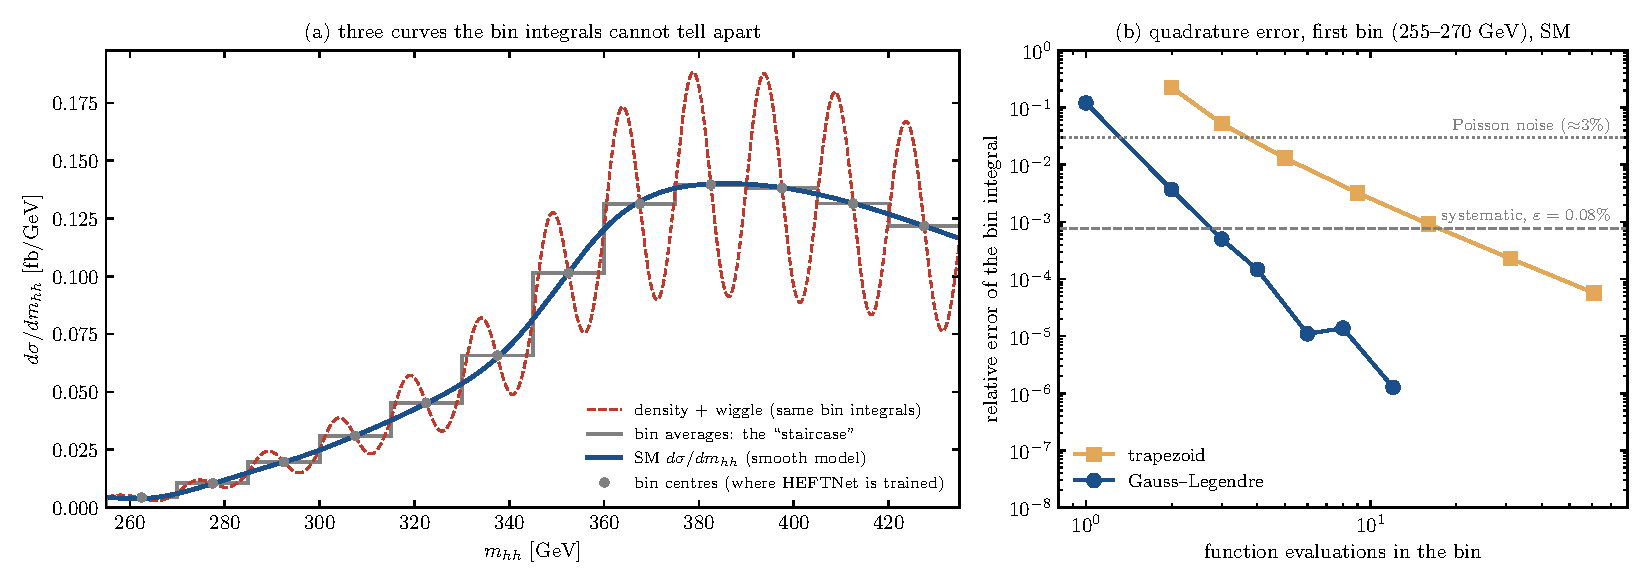
\includegraphics[width=\textwidth]{fig_density_plan.pdf}
\caption{(a) The SM density of the smooth model (blue), its bin averages (grey: the staircase a
network trained on bin values tends towards), and a density with a wiggle added in every bin
(red, dashed). All three have \emph{identical} bin integrals: the data cannot tell them apart.
(b) Relative error of the integral over the first bin, the hardest one, against the number of
function evaluations, for the trapezoid rule and Gauss--Legendre. The flattening of
Gauss--Legendre near $10^{-5}$ is a property of the test integrand: it is itself a cubic spline
with knots inside the bin. A smooth network has no such knots.}
\label{fig:plan}
\end{figure}

% ===========================================================================
\section{The idea: a density, compared through its bin integrals}
\label{sec:idea}

The data are bin integrals, so the model should be a density and the loss should compare its
integrals with the data:
\begin{equation}
  f_k(\theta) = \int_{e_k}^{e_{k+1}} \frac{d\sigma}{dm}\,dm = \sum_{i=1}^{23} C_i(\theta)\,A_{ik},
  \qquad A_{ik} = \int_{e_k}^{e_{k+1}} a_i(m)\,dm .
  \label{eq:binint}
\end{equation}
This is what the smooth model does, with splines. Here the $a_i$ come from the network.
Statisticians call such a model, one where the observations are integrals (or sums) of an
unobserved smooth function, a \emph{composite link model}~\cite{eilers07}.

\begin{keyidea}[Why this is cheap]
The 23 functions $a_i$ depend on $m$ only, not on $\theta$. So at each step we evaluate the
network at a \emph{fixed} set of nodes, 8 per bin, 640 in all, and form the table $A_{ik}$
[80, 23]. Each row $(\theta_s, k)$ of the batch then needs only the dot product of $\bC(\theta_s)$
with row $k$ of that table. Today the network is evaluated once per batch row (2,048 times per
step). With the density model it is evaluated 640 times per step, whatever the batch size.
\end{keyidea}

\begin{figure}[h]
\centering
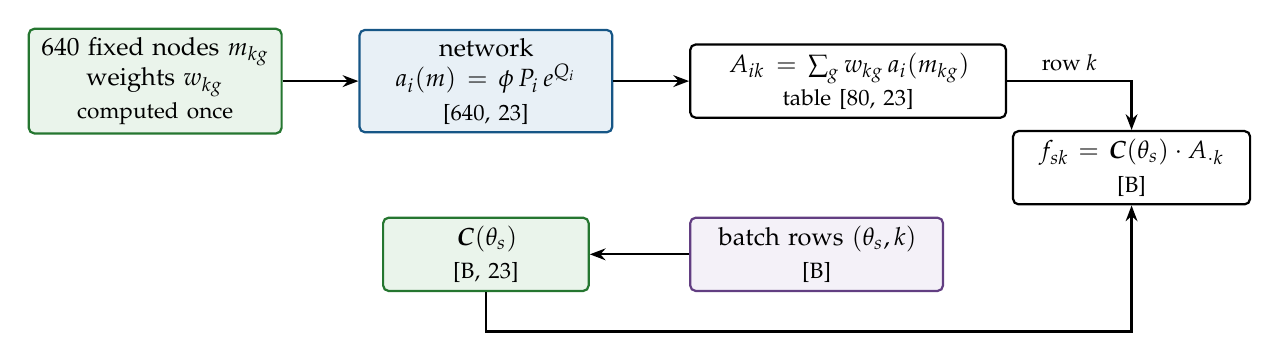
\begin{tikzpicture}[font=\small, >={Stealth[length=2mm]},
  box/.style={draw, rounded corners=2pt, thick, align=center, minimum height=9mm, inner sep=3pt},
  train/.style={box, fill=trainable!10, draw=trainable!80!black},
  phys/.style={box, fill=physics!10, draw=physics!80!black},
  dat/.style={box, fill=datac!8, draw=datac!80!black}]
\node[phys, text width=30mm] (nodes) at (0,0) {640 fixed nodes $m_{kg}$\\ weights $w_{kg}$\\[1pt]\footnotesize computed once};
\node[train, text width=30mm] (net) at (4.2,0) {network\\ $a_i(m)=\phi\,P_i\,e^{Q_i}$\\[1pt]\footnotesize [640, 23]};
\node[box, text width=38mm] (A) at (8.8,0) {$A_{ik}=\sum_g w_{kg}\,a_i(m_{kg})$\\[1pt]\footnotesize table [80, 23]};
\node[dat, text width=30mm] (rows) at (8.4,-2.2) {batch rows $(\theta_s, k)$\\[1pt]\footnotesize [B]};
\node[phys, text width=24mm] (C) at (4.2,-2.2) {$\bC(\theta_s)$\\[1pt]\footnotesize [B, 23]};
\node[box, text width=28mm] (f) at (12.4,-1.1) {$f_{sk}=\bC(\theta_s)\cdot A_{\cdot k}$\\[1pt]\footnotesize [B]};
\draw[->, thick] (nodes) -- (net);
\draw[->, thick] (net) -- (A);
\draw[->, thick] (rows) -- (C);
\draw[->, thick] (A.east) -| node[pos=0.25, above, font=\footnotesize]{row $k$} (f.north);
\draw[->, thick] (C.south) |- ++(0,-0.5) -| (f.south);
\end{tikzpicture}
\caption{The forward pass of the density model. Green: fixed (nodes, weights, monomials). Blue:
learned. The batch only selects rows of the table $A_{ik}$.}
\label{fig:forward}
\end{figure}

\paragraph{Units, and a warm start.} We let the network output $\hat a_i(m) = 15~\text{GeV}\times
a_i(m)$, the density ``per 15~GeV''. Then
\begin{equation}
  A_{ik} = \sum_g \frac{w_{kg}}{15~\text{GeV}}\,\hat a_i(m_{kg}) ,
\end{equation}
and $\hat a_i$ has the same size as today's network output. Any trained \code{HEFTNet}, e.g.\ the
Huber-fine-tuned \file{runs/FT_huber_d2}, can then be loaded into the density model as a
starting point (without $\phi$; \cref{sec:threshold}).

% ===========================================================================
\section{Gauss--Legendre quadrature, from the beginning}
\label{sec:gl}

\subsection{The idea}

A quadrature rule approximates an integral by a weighted sum of function values:
\begin{equation}
  \int_{-1}^{1} f(x)\,dx \approx \sum_{g=1}^{n} w_g\, f(x_g).
\end{equation}
The trapezoid rule fixes the nodes $x_g$ (equally spaced) and chooses only the weights. That
leaves $n$ free numbers, enough to integrate polynomials of degree $n-1$ exactly; in practice
the composite trapezoid rule is exact only for straight lines, and its error falls like $h^2$
with the spacing $h$. Gauss's idea (1814) was to choose the nodes \emph{as well}. With $2n$ free
numbers one can hope to integrate exactly all polynomials of degree $2n-1$, and this is possible.

\begin{aside}[Why $n$ nodes integrate degree $2n-1$ exactly]
Let $P_n$ be the Legendre polynomial of degree $n$. The Legendre polynomials are
\emph{orthogonal} on $[-1,1]$: $\int_{-1}^1 P_n\,q\,dx = 0$ for every polynomial $q$ of degree
less than $n$. Take the nodes $x_g$ to be the $n$ zeros of $P_n$, and the weights $w_g$ to be the
integrals of the Lagrange interpolating polynomials through those nodes, so that the rule is
exact for every polynomial of degree $\le n-1$.

Now take any polynomial $p$ of degree $\le 2n-1$ and divide it by $P_n$: $p = q\,P_n + r$, where
the quotient $q$ and the remainder $r$ both have degree $\le n-1$. Then:
\begin{itemize}
  \item exactly: $\int p\,dx = \int q P_n\,dx + \int r\,dx = 0 + \int r\,dx$, by orthogonality;
  \item by the rule: $\sum_g w_g\,p(x_g) = \sum_g w_g\,r(x_g)$, because $P_n(x_g) = 0$ at every node;
  \item and $\sum_g w_g\,r(x_g) = \int r\,dx$, because the rule is exact for degree $\le n-1$.
\end{itemize}
So the rule gives $\int p\,dx$ exactly. For a smooth $f$ the error is
\begin{equation}
  E_n = \frac{(b-a)^{2n+1}(n!)^4}{(2n+1)\,[(2n)!]^3}\,f^{(2n)}(\xi), \qquad \xi\in(a,b),
\end{equation}
against $-\frac{(b-a)\,h^2}{12} f''(\xi)$ for the composite trapezoid rule with spacing $h$.
\end{aside}

\subsection{Computing nodes and weights in PyTorch: the Golub--Welsch method}

PyTorch has \code{torch.trapezoid} but no Gauss--Legendre routine. We do not need one: the
nodes and weights are computed \emph{once}, before training, and then sit on the GPU as two
constant tensors. They can nevertheless be computed in PyTorch, in a few lines, by the method
of Golub and Welsch~\cite{golubwelsch}.

\begin{aside}[Nodes as eigenvalues]
Orthonormal polynomials obey a three-term recurrence. For the normalised Legendre polynomials
$p_k$ it reads
\begin{equation}
  x\,p_k(x) = \beta_{k+1}\,p_{k+1}(x) + \beta_k\,p_{k-1}(x), \qquad \beta_k = \frac{k}{\sqrt{4k^2-1}} .
\end{equation}
Write it for $k = 0,\dots,n-1$ as a matrix equation for the vector
$\boldsymbol p = (p_0,\dots,p_{n-1})$:
\begin{equation}
  x\,\boldsymbol p(x) = J\,\boldsymbol p(x) + \beta_n\,p_n(x)\,\boldsymbol e_n ,
\end{equation}
where $J$ is the symmetric tridiagonal matrix with zeros on the diagonal and
$\beta_1,\dots,\beta_{n-1}$ beside it, and $\boldsymbol e_n$ is the last unit vector. At a zero
$x_g$ of $p_n$ the last term vanishes, leaving $J\,\boldsymbol p(x_g) = x_g\,\boldsymbol p(x_g)$:
\textbf{the nodes are the eigenvalues of $J$}. One can show that the weights are $w_g = 2\,v_{1g}^2$,
where $v_{1g}$ is the first component of the normalised eigenvector $g$, and 2 is
$\int_{-1}^1 dx$.
\end{aside}

\begin{lstlisting}
import torch

def gauss_legendre(n, dtype=torch.float64):
    '''n-point Gauss-Legendre nodes x and weights w on [-1, 1] (Golub-Welsch).'''
    k   = torch.arange(1, n, dtype=dtype)
    b   = k / torch.sqrt(4 * k**2 - 1)            # beta_1 ... beta_{n-1}
    J   = torch.diag(b, 1) + torch.diag(b, -1)    # symmetric tridiagonal matrix
    x, V = torch.linalg.eigh(J)                   # eigenvalues (sorted), eigenvectors
    w   = 2 * V[0]**2                             # first component of each eigenvector
    return x, w

def bin_nodes(edges, n=8):
    '''Nodes m [K*n] and weights w [K*n] for the bins [edges[k], edges[k+1]].'''
    x, w = gauss_legendre(n)
    e = torch.as_tensor(edges, dtype=torch.float64)
    c, h = 0.5 * (e[1:] + e[:-1]), 0.5 * (e[1:] - e[:-1])  # centres, half-widths
    m  = (c[:, None] + h[:, None] * x[None]).reshape(-1)   # map [-1,1] onto each bin
    wt = (h[:, None] * w[None]).reshape(-1)                # dm = h dx
    return m, wt
\end{lstlisting}

The computation is done in double precision, so the nodes and weights are exact to the last
bit, and then converted to float32. We will check them against \code{numpy.polynomial.legendre.leggauss}
(agreement to $10^{-15}$) and against exact integrals of polynomials of degree $2n-1$.

\subsection{How many nodes?}

\Cref{fig:plan}b and \cref{tab:quad} show the relative error of the bin integral for realistic
integrands, the smooth model's own densities. The first bin is the hardest, because the threshold
factor $\phi = \sqrt{1-4m_h^2/m^2}$ bends sharply there: $|\phi''/\phi| \approx 0.01~\text{GeV}^{-2}$
at 255~GeV.

\begin{table}[h]
\centering
\small
\setlength{\tabcolsep}{4pt}
\begin{tabular}{llcccccc}
\toprule
 & & \multicolumn{3}{c}{trapezoid, sub-intervals per bin} & \multicolumn{3}{c}{Gauss--Legendre, nodes per bin}\\
spectrum & bin (GeV) & 1 & 4 & 15 & 2 & 4 & 8\\
\midrule
SM & 255--270 & 23\% & 1.3\% & 0.09\% & 0.4\% & 0.015\% & 0.0014\%\\
SM & 300--315 & 0.6\% & 0.04\% & 0.003\% & 0.01\% & $3\times10^{-6}$ & $2\times10^{-7}$\\
most cancelling (ID 917) & 255--270 & 26\% & 1.4\% & 0.10\% & 0.6\% & 0.028\% & 0.0025\%\\
most cancelling (ID 917) & 300--315 & 2.6\% & 0.10\% & 0.007\% & 0.24\% & 0.006\% & 0.0003\%\\
\bottomrule
\end{tabular}
\caption{Relative error of the integral over one bin, for the smooth model's density. For
comparison: Poisson noise near threshold $\approx 3\%$; the systematic $\varepsilon \approx 0.08\%$.}
\label{tab:quad}
\end{table}

\begin{watch}[Why the quadrature must be better than the noise]
The loss never sees the exact integrals, only the quadrature sums. The network will learn
whatever density makes the \emph{sums} match POWHEG. A quadrature error therefore does not show
up in the loss or in the bin predictions; it shows up as a bias in the learned density. With 8
Gauss--Legendre nodes per bin the error is below $3\times10^{-5}$ in every case tested, well below the
systematic floor. The trapezoid rule would need about 1~GeV spacing near threshold just to reach
the floor ($\approx 10^{-3}$, column ``15''). An earlier estimate of mine in the chat
(0.03\% at 1~GeV) was too optimistic by a factor of 3.
\end{watch}

\textbf{Proposal:} 8 Gauss--Legendre nodes in every bin (640 nodes), and a check that 16 nodes
change nothing.

% ===========================================================================
\section{The threshold factor}
\label{sec:threshold}

At $m = 2m_h = 250$~GeV the two-body phase space closes, and $d\sigma/dm$ vanishes like the Higgs
velocity in the $hh$ rest frame, $\phi(m) = \sqrt{1-4m_h^2/m^2}$. Today's network has no reason
to know this. Multiplying by $\phi$,
\begin{equation}
  \hat a_i(m) = \phi(m)\,P_i(x)\,e^{Q_i(x)},
\end{equation}
leaves the network only the smooth remainder to describe. For the spline model this changed
nothing inside 255--1455~GeV, but made the extrapolation to 240--255~GeV 8\% high instead of
55\% high. With $\phi$ on, a warm start from an existing network is poor near threshold (there
$\phi \approx 0.2$--0.5), so training should start from scratch. With $\phi$ off, the warm start
is a quick first test.

% ===========================================================================
\section{The activation: smoothness of the density}
\label{sec:activation}

\subsection{ReLU gives kinks}

$P$ is a network of one input. With ReLU, each hidden unit is either off or linear in its input,
so $P_i(x)$ is \emph{piecewise linear} in $x$, with a kink wherever a unit switches. The final
$\tanh$ and the envelope $e^{Q}$ round the kinks somewhat, but the derivative of $d\sigma/dm$
still jumps at places chosen by the training, not by the physics. For bin integrals this hardly
matters. For a density meant to be read between bin centres, and differentiated, it does.

\subsection{Smooth alternatives}

\begin{center}
\small
\begin{tabular}{llp{7.6cm}}
\toprule
activation & smoothness & behaviour \\
\midrule
ReLU (today) & kinks & piecewise linear; baseline \\
tanh & smooth & saturates; classic choice for smooth regression \\
SiLU, $x/(1+e^{-x})$ & smooth & ReLU-like for large $x$, smooth near 0; trains like ReLU \\
sine & smooth, oscillatory & see below \\
\bottomrule
\end{tabular}
\end{center}

\paragraph{Sine.} \file{heftnet.py} already defines a \code{Sin} module, and \code{ACTIVATION = 'Sin'}
works with the architecture as it stands. Sine networks (``SIRENs''~\cite{siren}) are smooth to
all orders, and are popular because, with a frequency factor $\sin(30\,Wx)$ in the first layer
and a special initialisation, they represent fine detail very well. Fine detail is exactly what
we do \emph{not} want: a sine network can oscillate inside a bin at no cost in the loss
(\cref{sec:nullspace}). With PyTorch's default initialisation and no frequency factor the first
layer's weights lie in $(-1,1)$, and our input $x$ lies in $[0, 0.8]$, so the argument of each first-layer sine changes
by less than one radian across the whole mass range. The network then starts in the
low-frequency regime and behaves like a smooth basis, much like tanh. That is the regime we
propose. Training can raise the frequencies, which the curvature penalty of the next section
guards against. Outside the training range a sine network keeps oscillating, another reason not
to use the network beyond 1455~GeV.

\textbf{Proposal:} a switch \code{ACTIVATION} $\in$ \{\code{'nn.ReLU'}, \code{'Sin'}, \code{'nn.Tanh'},
\code{'nn.SiLU'}\}, all four trained and compared (\cref{sec:evaluation}).

% ===========================================================================
\section{What bin integrals cannot see, and a curvature penalty}
\label{sec:nullspace}

\subsection{The null space}

Take any function $u(m)$ whose integral over every bin is zero, for example
$u(m) = c_k\sin\!\big(2\pi(m-e_k)/15~\text{GeV}\big)$ in bin $k$. Adding $u$ to any $a_i$ changes
no prediction, no loss and no gradient. The red curve of \cref{fig:plan}a is such a case.
In linear-algebra language, $u$ is in the \emph{null space} of the map from densities to bin
integrals. The data say nothing about that part of the density. Something else must: the
smoothness of the model.

For the spline model the something else is explicit: the splines cannot oscillate faster than the
knot spacing, and the smoothness prior penalises curvature with a strength set by the evidence.
For the network it is implicit, in the architecture and the training, and therefore
uncontrolled. This is the deeper reason for the large spread of the ensemble between bin centres.

\subsection{A penalty on curvature}

We propose an explicit, optional penalty: on a uniform grid $m_j$ with spacing $h = 1$~GeV from
255 to 1455~GeV (1,201 points), the second differences
$\Delta^2 a_{ij} = a_i(m_{j+1}) - 2a_i(m_j) + a_i(m_{j-1}) \approx h^2 a_i''(m_j)$, and
\begin{equation}
  R_\text{curv} = \lambda\;\frac{1}{23}\sum_{i=1}^{23}
  \frac{\sum_j \big(L^2\,\Delta^2 a_{ij}/h^2\big)^2}{\sum_j a_{ij}^2},
  \qquad L = 100~\text{GeV}.
  \label{eq:curv}
\end{equation}
Each term is the mean squared curvature of $a_i$ on the scale $L$, relative to the size of $a_i$,
so that functions of very different sizes are treated alike and $\lambda$ is dimensionless. The
denominator is held fixed in each step (\code{detach}), so the penalty only discourages
curvature and does not shrink the functions. The wiggle of \cref{fig:plan}a has $L^2|a''|/|a|$ of
order $(2\pi L/15)^2 \approx 2\times10^3$; a physical $a_i$, varying on scales of 20--100~GeV, of
order 1--25. So a small $\lambda$ kills null-space wiggles while leaving the physics alone. This
is the network version of the spline model's P-spline prior~\cite{eilers96}. It costs 1,201
more evaluations of the one-input network per step.

\textbf{Proposal:} \code{CURV\_LAMBDA} $\in \{0, 10^{-4}, 10^{-3}, 10^{-2}\}$; adopt the largest
value that leaves the test-spectrum $-2\ln\lambda$ unchanged (within 0.005).

% ===========================================================================
\section{Training}
\label{sec:training}

Nothing about the data changes: the rows, the targets (pb per bin) and the splits are those of
\file{heft_train.ipynb}. Because the density model takes the same input rows $[N, 6]$ and returns
the same kind of output (pb per bin), the \code{drwho} datasets, loaders, monitor and
\code{compute\_avg\_loss}, and \code{finetune.finetune}, all work unchanged.

\begin{enumerate}
  \item \textbf{Stage 1}: Adam with the L1 loss, as now, from scratch (or warm start with $\phi$ off).
  \item \textbf{Stage 2}: the fine-tune (\file{heft_finetune.ipynb}) with the Huber loss of the pulls,
    with \code{variance\_from='model'}, i.e.\ the Poisson variance of the model's prediction.
    Weighting by the observed counts biases fits low (\file{docs/smooth/smooth_results.pdf}),
    and this was never done for the networks.
  \item The curvature penalty, if used, is added to the loss in both stages.
\end{enumerate}
The bin index $k$ of a row is recovered from its input $x$ as $k = \mathrm{round}(100x - 0.5)$,
exactly as in \file{heft_smooth.ipynb}.

% ===========================================================================
\section{Code}
\label{sec:code}

\begin{itemize}
  \item \textbf{New module \file{dihiggs/quadrature.py}}: \code{gauss\_legendre(n)} and
    \code{bin\_nodes(edges, n)} as above, with tests.
  \item \textbf{New class \code{HEFTDensity} in \file{dihiggs/heftnet.py}}, a subclass of
    \code{HEFTNet}, so that every saved \code{HEFTNet} still loads as before:
\end{itemize}
\begin{lstlisting}
class HEFTDensity(HEFTNet):
    '''HEFTNet as a density: forward(x) returns the INTEGRAL over the bin of x.'''
    def __init__(self, n_nodes=8, threshold=True,
                 edges=255.0 + 15.0 * np.arange(81), **kw):
        super().__init__(**kw)
        m, w = bin_nodes(edges, n_nodes)
        # register_buffer: tensors that move with model.to(device) and are saved
        # with the model, but are not trained
        self.register_buffer('m_nodes', m.float())
        self.register_buffer('w_nodes', (w / 15.0).float())   # output is "per 15 GeV"
        self.n_bins, self.n_nodes, self.threshold = len(edges) - 1, n_nodes, threshold

    def density15(self, m):
        '''15 GeV x a_i(m) at the masses m (GeV): [len(m), 23].'''
        a = self.coeffs((m - 255.0) / 1500.0)          # P * exp(Q), as before
        if self.threshold:
            a = a * torch.sqrt(1 - 4 * 125.0**2 / m**2)[:, None]
        return a

    def forward(self, x):
        # 1. the table of bin integrals A [n_bins, 23], from the fixed nodes
        a = self.density15(self.m_nodes) * self.w_nodes[:, None]
        A = a.view(self.n_bins, self.n_nodes, 23).sum(dim=1)
        # 2. each row picks its bin k and its 23 monomials C_i(theta)
        k = torch.round(x[:, 0] * 100 - 0.5).long()
        C = self.monomials(x[:, 1:])                      # the 23 C_i(theta), [B, 23]
        return (C * A[k]).sum(dim=1)
\end{lstlisting}
\begin{itemize}
  \item The monomials, now written inside \code{HEFTNet.forward}, move to a method
    \code{monomials(theta)} that both classes use (no change in behaviour; checked against
    \code{smooth.heft\_monomials}).
  \item A method \code{dsigma\_dm(theta, m)} for the density at any $m$, used by
    \file{heft_test.ipynb}, the figures, and \code{smooth\_common.network\_density}.
  \item \textbf{Notebooks}: switches in \file{heft_train.ipynb} and \file{heft_finetune.ipynb}
    (\cref{tab:switches}); run folders \file{runs/DENS_<activation>[_thr][_curv<lambda>]}.
\end{itemize}

\begin{table}[h]
\centering
\small
\begin{tabular}{lll}
\toprule
switch & values & meaning\\
\midrule
\code{MODEL} & \code{'bins'}, \code{'density'} & today's \code{HEFTNet}, or \code{HEFTDensity}\\
\code{N\_NODES} & 8 (16 as a check) & Gauss--Legendre nodes per bin\\
\code{THRESHOLD} & \code{True}, \code{False} & multiply by $\phi(m)$\\
\code{ACTIVATION} & \code{'nn.ReLU'}, \code{'Sin'}, \code{'nn.Tanh'}, \code{'nn.SiLU'} & hidden-layer activation\\
\code{CURV\_LAMBDA} & 0, $10^{-4}$, $10^{-3}$, $10^{-2}$ & curvature penalty \cref{eq:curv}\\
\code{WARM\_START} & \code{None} or a parameter file & initialise from a trained \code{HEFTNet}\\
\bottomrule
\end{tabular}
\caption{Notebook switches.}
\label{tab:switches}
\end{table}

% ===========================================================================
\section{Tests and evaluation}
\label{sec:evaluation}

\paragraph{Before any training: a toy with a known answer.} \file{code/smooth_toy.py} generates
spectra of 40,000 Poisson events from three known smooth coefficient functions. We train the
density network on its bins and compare the learned $a_i(m)$ with the truth \emph{between} bin
centres, together with a bin-value network as the contrast. This tests the whole idea where the
answer is known.

\paragraph{On the POWHEG spectra.}
\begin{enumerate}
  \item \textbf{Accuracy}: mean $-2\ln\lambda$ per bin on the 1,000 test spectra, below and above
    555~GeV, against the smooth model (1.566, 1.100) and the bin-value network (1.561, 1.121).
  \item \textbf{Calibration}: pulls with the model-error term, overall and by cancellation fifth.
  \item \textbf{Inside a bin, the merged-bin test}: train on the training spectra merged into 30~GeV
    bins (merging pairs of rows of a spectrum adds their counts, so the data stay Poisson; the
    density model just uses 30~GeV edges), predict the 15~GeV bins of the test spectra. The
    spline model passes above 360~GeV ($\chi^2 \approx 1$); a bin-value model cannot.
  \item \textbf{Between bin centres}: an ensemble of 10 seeds for the best configuration; the
    relative spread of $d\sigma/dm$ between centres, against that at the centres
    (\file{fig_interpolation} updated).
  \item \textbf{Against the spline model}: $d\sigma/dm$ and the $a_i(m)$ of the two models on a
    0.5~GeV grid.
  \item \textbf{Checks}: 8 against 16 nodes; the extrapolation to 240--255~GeV with $\phi$.
\end{enumerate}

\begin{keyidea}[Success criteria]
Accuracy no worse than today's network; the merged-bin test passed above 360~GeV, like the
spline model; the ensemble spread between bin centres no larger than at the centres; and a
density that agrees with the spline model's within the two models' uncertainties.
\end{keyidea}

% ===========================================================================
\section{Order of work}
\label{sec:order}

\begin{enumerate}
  \item \file{quadrature.py} and its tests; \code{monomials()} refactor; \code{HEFTDensity}; a test that
    \code{forward} equals the bin integrals of \code{dsigma\_dm} computed independently (CPU, here).
  \item The toy (CPU or the 5090).
  \item Notebook switches; one short run per activation with $\phi$ on and \code{CURV\_LAMBDA} = 0
    to check that training is stable (5090).
  \item The grid: 4 activations $\times$ \{$\phi$ on\} $\times$ 4 values of $\lambda$, stage 1 + stage 2
    (5090; each run as long as today's).
  \item Merged-bin test and ensemble for the best configuration; figures; a short results note.
\end{enumerate}

% ===========================================================================
\section{Decisions for you}
\label{sec:decisions}

\begin{keyidea}[Decisions before I proceed]
\begin{enumerate}
  \item \textbf{Gauss--Legendre with 8 nodes per bin}, computed in PyTorch by Golub--Welsch,
    rather than the trapezoid rule. Agreed?
  \item \textbf{Network output ``per 15~GeV''} ($\hat a_i = 15~\text{GeV}\times a_i$), so that
    existing networks can serve as a warm start. Agreed?
  \item \textbf{Threshold factor $\phi$ on} by default, training from scratch. Agreed?
  \item \textbf{Activations}: compare ReLU, sine (low frequency, default initialisation), tanh and
    SiLU. Any to add or drop?
  \item \textbf{Curvature penalty} \cref{eq:curv} with a scan of $\lambda$. Agreed, or would you
    rather start without it?
  \item \textbf{Code layout}: new \file{dihiggs/quadrature.py}; \code{HEFTDensity} as a subclass in
    \file{heftnet.py}; switches in the existing \file{heft_train.ipynb} and
    \file{heft_finetune.ipynb} rather than new notebooks. Acceptable?
  \item \textbf{The toy test first}, before any POWHEG run. Agreed?
\end{enumerate}
\end{keyidea}


% ===========================================================================
\section{Addendum (4 November): decisions, and what the toy test changed}
\label{sec:addendum}

\paragraph{Decisions.} (1) Gauss--Legendre, 8 nodes per bin. (2) The network models the density
$a_i(m)$ itself, in pb/GeV; no warm start from the trained networks, so the ``per 15~GeV''
convention of \cref{sec:idea} is dropped. (3) Threshold factor on. (4) ReLU dropped; SiLU is
the default, tanh and sine are options. (5) No curvature penalty for now. (6) Code layout as
proposed. (7) The toy test first.

\paragraph{Two changes forced by the toy} (\file{code/density_toy.py}).
\begin{enumerate}
  \item \textbf{The network's input variable.} With HEFTNet's $x = (m-255)/1500$ the density
    network could not fit the threshold region: $\chi^2$ per bin of 6--13 in the first four bins,
    1.7 overall. All the structure of 255--435~GeV lies in the first 12\% of the range of $x$, and
    a smooth network cannot bend that sharply there. With
    \begin{equation}
      z = 2\sqrt{\frac{m - 250~\text{GeV}}{1205~\text{GeV}}} - 1 ,
    \end{equation}
    which, like the spline knots, gives 255--435~GeV a third of the input range, $\chi^2$ per bin
    is $\approx 1$ in every bin. This is now the default (\code{input\_map='sqrt'}).
  \item \textbf{The optimiser.} Full-batch Adam converges slowly on this problem ($\chi^2$ per bin
    1.74 after 15,000 steps). L-BFGS, a quasi-Newton method, converges in about a minute on a
    laptop, but only in double precision: in single precision its line search stalls. A full-batch
    evaluation of the density model is cheap (the network sees only the 640 nodes), so L-BFGS is
    practical here. New: \code{finetune.finetune\_lbfgs} and the switch \code{OPTIMIZER='lbfgs'} in
    \file{heft_finetune.ipynb}.
\end{enumerate}

\paragraph{Toy results.} Three seeds per model; all reach $\chi^2$ per bin $\approx 1$. The
``bins'' model is the same network with the bin integral replaced by 15~GeV times the value at the
bin centre (a 1-node rule), which is what HEFTNet assumes.

\begin{center}
\small
\begin{tabular}{lcccc}
\toprule
 & \multicolumn{3}{c}{r.m.s.\ error of $a_i(m)$ / max$|a_i|$ (\%)} & bias, 255--285 GeV (\%)\\
model & 0.5 GeV grid & bin centres & 255--345 GeV & mean $\pm$ s.d.\ of seeds\\
\midrule
density, SiLU & 0.53 & 0.53 & 1.02 & $+0.07 \pm 0.07$\\
density, tanh & 0.51 & 0.51 & 1.09 & \\
density, sine & 0.36 & 0.36 & 0.93 & $+0.38 \pm 0.25$\\
bins (1 node), SiLU & 0.69 & 0.70 & 1.58 & $+0.46 \pm 0.04$\\
spline model (reference) & 0.16 & 0.16 & 0.44 & $+0.16$\\
\bottomrule
\end{tabular}
\end{center}

\begin{watch}[What the toy does and does not show]
\begin{itemize}
  \item The plan's criterion, a density network at least twice as accurate as the bin-value
    network, is \textbf{not} met in this toy: with a smooth activation, the square-root input and a
    good optimiser, the bin-value network is only modestly worse (0.69\% against 0.53\%). Neither
    shows a larger error between bin centres than at them. The toy is too easy to reproduce the
    spread of the old ensemble between centres; the factorial test below, on a realistic toy, does.
  \item What the integral removes is a \textbf{bias} where the density is curved: near threshold
    the bin-value network is wrong by $+0.46\%$, the same in every seed (12 times their spread);
    the density network is unbiased there. In the toy the threshold curvature is mild. For POWHEG
    it is larger: for the SM, 15~GeV times the density at the centre of the first bin is 12\% below
    the bin integral, so the bias of a bin-value model will matter there.
  \item The networks are 2--3.5 times less accurate than the spline model, which has a smoothness
    prior; their errors are smooth waves on scales of about 100~GeV, in the combinations of the
    $a_i$ that the toy's three monomials determine least well.
\end{itemize}
\end{watch}


\paragraph{Factorial test} (\file{code/density_ablation.py}). To find what caused the old ensemble's
spread between bin centres, and whether the density target pays off, the same network was trained
with each ingredient changed separately.

\emph{Simple toy} (the toy above; 9 configurations, 3 seeds each, all trained to convergence the same
way). No configuration, the exact old one included (ReLU, linear input, bin values, no $\phi$:
$\chi^2$ per bin 0.997), shows a larger seed spread between bin centres than at them (ratio
0.93--1.14). In an easy problem, neither ReLU nor the linear input makes the network wiggle.

\emph{Realistic toy.} The truth is the spline model's own 23 $a_i(m)$ (\file{runs/SMOOTH_J40}), at
1,500 HEFT points of the real training spectra, with 40,000 Poisson events per spectrum: real
threshold curvature and real cancellations, and a known answer. Every configuration was trained with
the production recipe (L1, mini-batch Adam, 200,000 steps; then the Huber fine-tune with Poisson
variances, full-batch Adam, 10,000 steps); with a short recipe this toy does not converge from a random
start. Two seeds each; all reach $\chi^2$ per bin 0.97 on the training spectra. The density
$d\sigma/dm$ was compared with the truth at 300 HEFT points on a 0.5~GeV grid:

\begin{center}
\footnotesize
\setlength{\tabcolsep}{3pt}
\begin{tabular}{lcccc}
\toprule
 & \multicolumn{2}{c}{r.m.s.\ error / peak (\%)} & bias, 255--285 GeV & max seed spread (\% of peak),\\
configuration & 255--600 GeV & 255--345 GeV & (\% of local density) & between / at centres, 255--600 GeV\\
\midrule
old: ReLU, linear, bins, no $\phi$ & 1.62 & 3.00 & $-0.44 \pm 0.23$ & 2.40 / 0.22\\
SiLU, linear, bins, no $\phi$ & 0.53 & 1.00 & $-0.79 \pm 0.04$ & 1.11 / 0.07\\
SiLU, sqrt input, bins, $\phi$ & 0.54 & 1.04 & $-1.13 \pm 0.01$ & 0.30 / 0.06\\
\textbf{SiLU, sqrt input, density, $\phi$} & \textbf{0.28} & \textbf{0.50} & $\mathbf{-0.02 \pm 0.01}$ & \textbf{0.21 / 0.09}\\
\bottomrule
\end{tabular}
\end{center}

\begin{keyidea}[What the factorial test shows]
\begin{itemize}
  \item \textbf{The realistic toy reproduces the old wiggles}: for the old configuration the seeds
    agree to 0.13\% (of the local density) at the bin centres and differ by up to 4.8\% between them,
    as in \file{docs/paper/fig_interpolation.pdf} (0.19\% and 4.4\%).
  \item \textbf{Their causes, in order}: the linear input together with no threshold factor (the
    maximum spread between centres falls from 1.1\% to 0.30\% of the peak), ReLU (from 2.4\% to 1.1\%),
    and the bin-value target (from 0.30\% to 0.21\%). ReLU is a cause, but not the main one.
  \item \textbf{The density target halves the error} of the best bin-value network (0.28\% against 0.54\%
    of the peak density below 600~GeV; 0.50\% against 1.04\% near threshold), and \textbf{removes a bias}
    of $-1.1\%$ near threshold, the same in both seeds. The seeds agree far better than either agrees
    with the truth: the bin-value network's error is systematic, the misreading of bin contents as
    densities, not noise.
  \item SiLU is three times more accurate than ReLU with the old input (1.62\% against 0.53\%).
\end{itemize}
Caveats: two seeds; the truth is itself a spline times $\phi$, which favours the $\phi$ and
square-root-input configurations somewhat; the toy has no model error, unlike POWHEG; ReLU with the
square-root input was not run.
\end{keyidea}

\paragraph{Next} (on the 5090): \file{heft_train.ipynb} with \code{MODEL='density'} (L1, Adam), then
\file{heft_finetune.ipynb} with \code{VARIANCE\_FROM='model'} and the default \code{OPTIMIZER='adam'} (the recipe
tested on the realistic toy; L-BFGS remains an option); compare with
the spline model on the test spectra (\cref{sec:evaluation}).

% ===========================================================================
\begin{thebibliography}{9}
\bibitem{eilers07} P.~H.~C.~Eilers, \emph{Ill-posed problems with counts, the composite link
  model and penalized likelihood}, Statistical Modelling \textbf{7} (2007) 239.
\bibitem{golubwelsch} G.~H.~Golub and J.~H.~Welsch, \emph{Calculation of Gauss quadrature rules},
  Math.\ Comp.\ \textbf{23} (1969) 221.
\bibitem{siren} V.~Sitzmann, J.~N.~P.~Martel, A.~W.~Bergman, D.~B.~Lindell and G.~Wetzstein,
  \emph{Implicit neural representations with periodic activation functions}, NeurIPS 2020,
  \href{https://arxiv.org/abs/2006.09661}{arXiv:2006.09661}.
\bibitem{eilers96} P.~H.~C.~Eilers and B.~D.~Marx, \emph{Flexible smoothing with B-splines and
  penalties}, Statist.\ Sci.\ \textbf{11} (1996) 89.
\end{thebibliography}

\end{document}
